\section{Introduction}
%\subsection{Clinical Context}
Glomerular disease is a significant health issue affecting the kidneys, which are essential organs responsible for filtering blood, removing waste, and maintaining electrolyte balance \cite{thomas2006renal}.
Each kidney contains approximately one million nephrons, the functional units that filter blood. 
Within each nephron, the glomerulus acts as a critical filtration barrier, preventing large molecules such as proteins and blood cells from passing into the urine while allowing waste products and excess substances to be excreted \cite{clevelandclinic}.

%Glomerular diseases are a major cause of chronic kidney disease (CKD), affecting about 10\% of the global population \cite{clinical_context}. 
%Damage to the glomeruli can result from various etiologies, including autoimmune disorders, hereditary conditions, infections, and sclerotic diseases. 
%Persistent glomerular inflammation can lead to scarring, known as glomerulosclerosis, which further impairs kidney function.

Glomerular diseases, a major cause of chronic kidney disease (CKD) that affects about 10\% of the global population \cite{clinical_context}, can compromise the kidneys' ability to filter blood properly, leading to progressive kidney damage if left untreated \cite{clevelandclinic}.
On the other hand, early detection and treatment of glomerular diseases can be crucial to prevent kidney damage and maintain overall health. 
In this context, the analysis of kidney pathology images has become increasingly important, particularly segmenting glomeruli from Whole Slide Images (WSIs).


Accurate segmentation is essential for diagnosing glomerular diseases, as it allows clinicians to assess the extent of glomerular damage, evaluate treatment efficacy, and study disease progression  \cite{kaur2023automatic,jha2021instance} .
Historically, the task has been performed manually by pathologists, a process that is both time-consuming and prone to variability \cite{jiang_deep_2021}. 
Early automated methods relied on classical image processing techniques such as thresholding, edge detection, and template matching, but these approaches struggled with the complex variability in glomeruli shapes and tissue appearances. 
More recent advances in deep learning have revolutionized glomeruli segmentation, offering the ability to learn rich representations from labeled data, providing more precise and scalable solutions \cite{bouteldja2021deep,lutnick_user-friendly_2022,leng_accelerated_2023}.

\subsection*{The KPIs challenge}
The \textbf{MICCAI 2024 Kidney Pathology Image Segmentation (KPIs) Challenge} was organized to explorethe boundaries of glomeruli segmentation through a competitive framework. 
Participants were tasked with developing segmentation algorithms to accurately identify glomeruli from WSIs in various CKD contexts. 
The challenge emphasized the importance of segmenting glomeruli at a pixel level, which is useful for enabling a better understanding of CKD development. 
The organization made available a dataset with a wide range of image variations such as large differences in glomeruli size, shape, and structural changes due to disease states or tissue preparation techniques \cite{KPIs2024}.
The challenge is divided into two distinct tasks:
\begin{enumerate}
    \item \textbf{Patch-level Segmentation:} This task focused on segmenting glomeruli from smaller, predefined patches of the WSI. 
    The goal was to isolate glomeruli accurately within these constrained regions, often used for training deep learning models due to the reduced computational load and focused analysis.
    \item \textbf{Whole Slide Image Segmentation:} This task required to segment glomeruli across entire slide images, offering a more comprehensive view of the tissue. 
WSIs present additional challenges due to their large size and the diversity of tissue types, demanding algorithms that can generalize well across different CKD disease models and tissue conditions.
\end{enumerate}

\begin{figure}[!t]
\centering
\subfloat[]{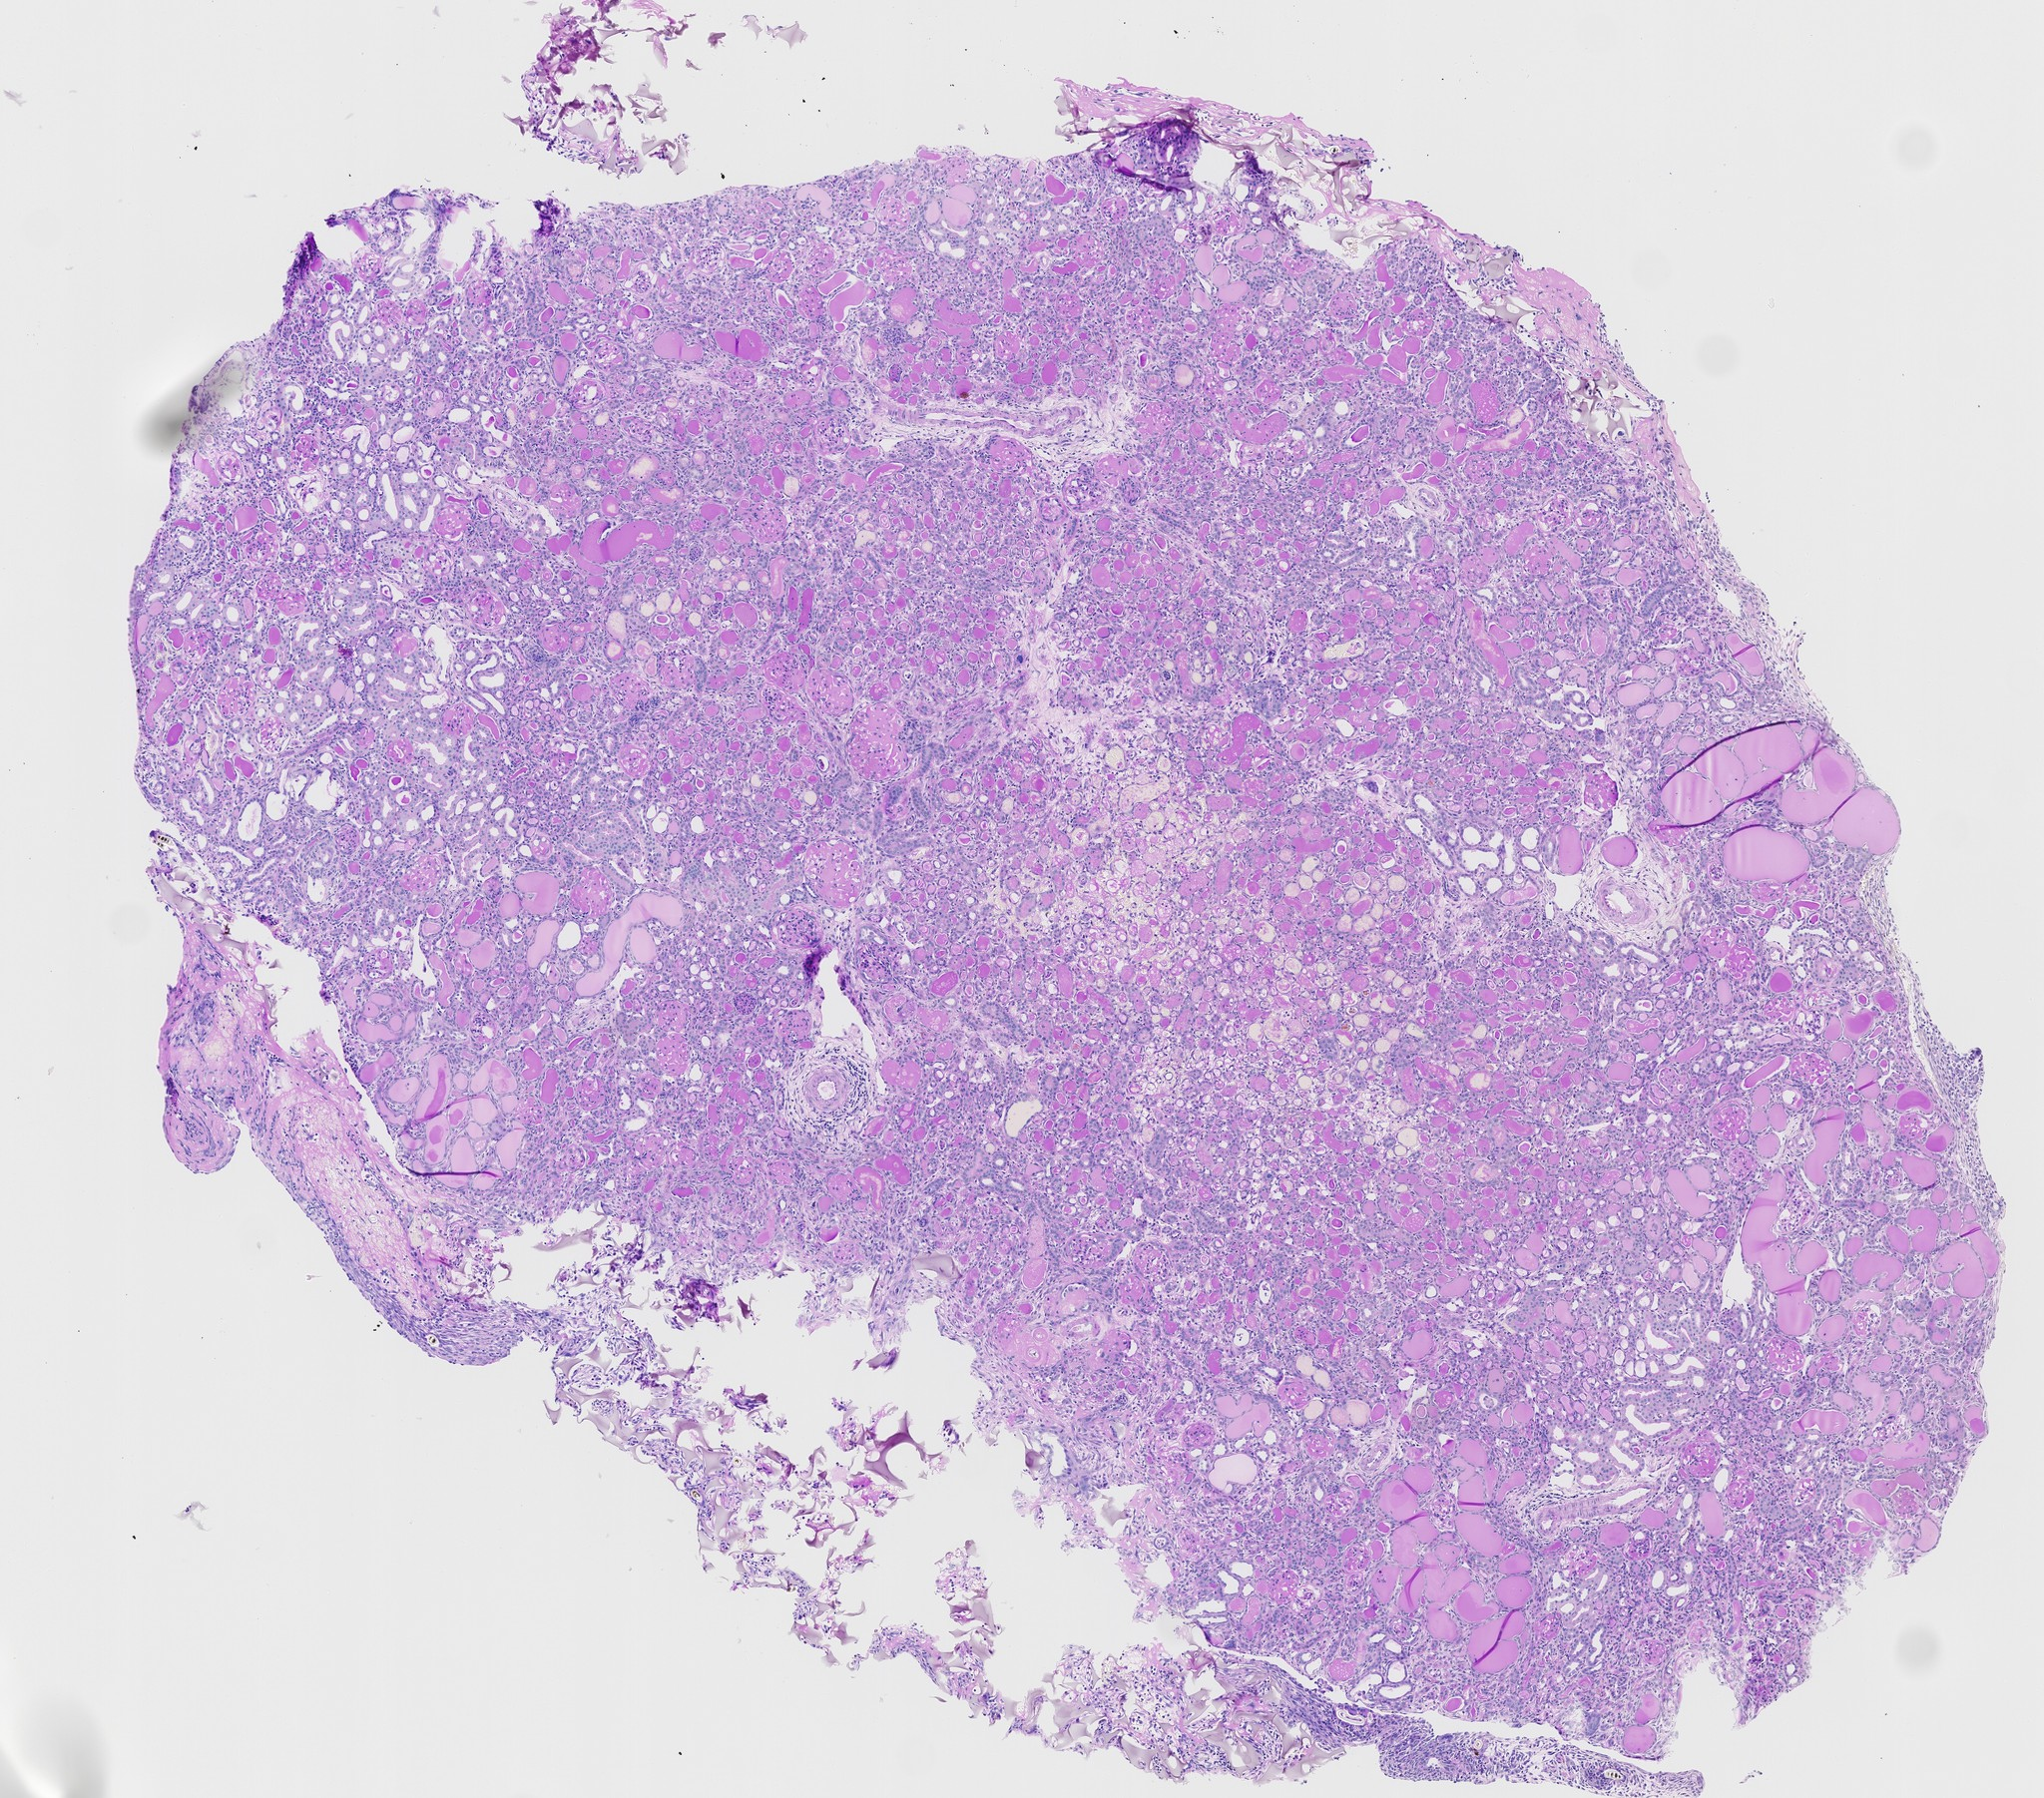
\includegraphics[width = 0.24\textwidth,valign=c]{images/08-373_03_wsi.jpg}
\label{fig_o1}}
\hfil
\subfloat[]{\includegraphics[width = 0.24\textwidth,valign=c]{images/08-373_03_mask.png}
\label{fig_o2}}
\hfil
\subfloat[]{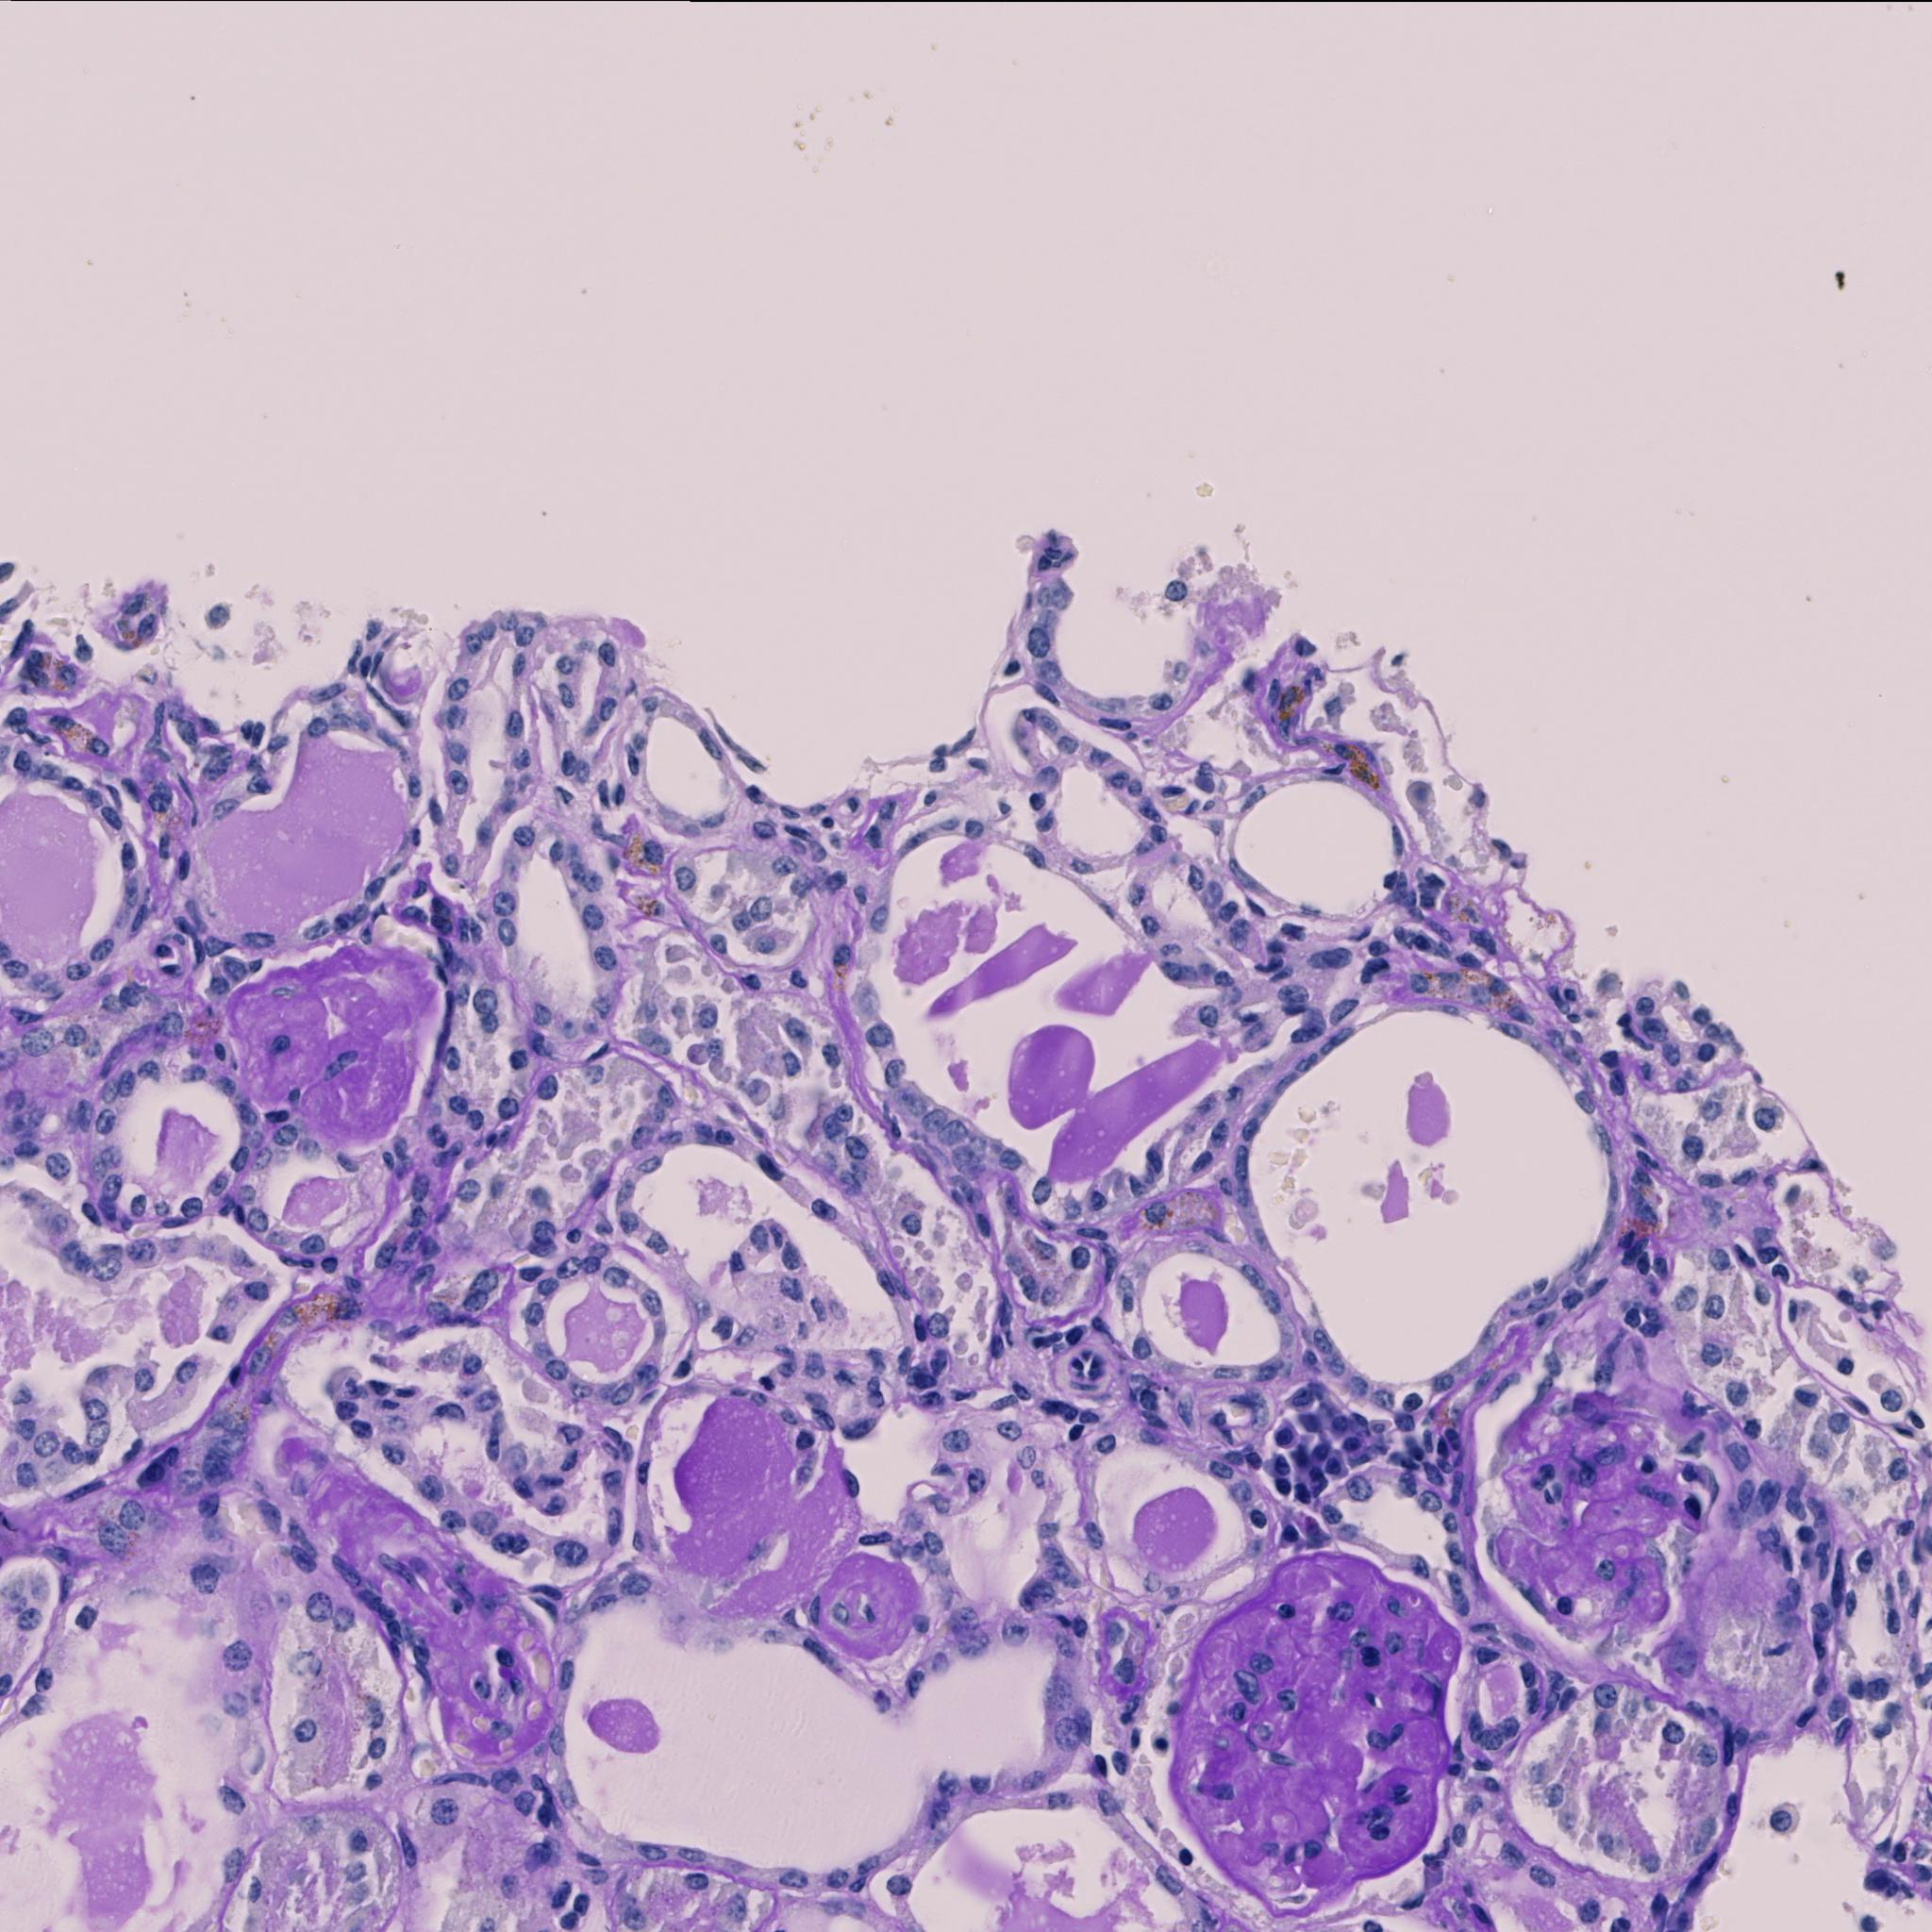
\includegraphics[width = 0.24\textwidth,valign=c]{images/56Nx_12_116_5_5120_0_img.jpg}
\label{fig_o3}}
\hfil
\subfloat[]{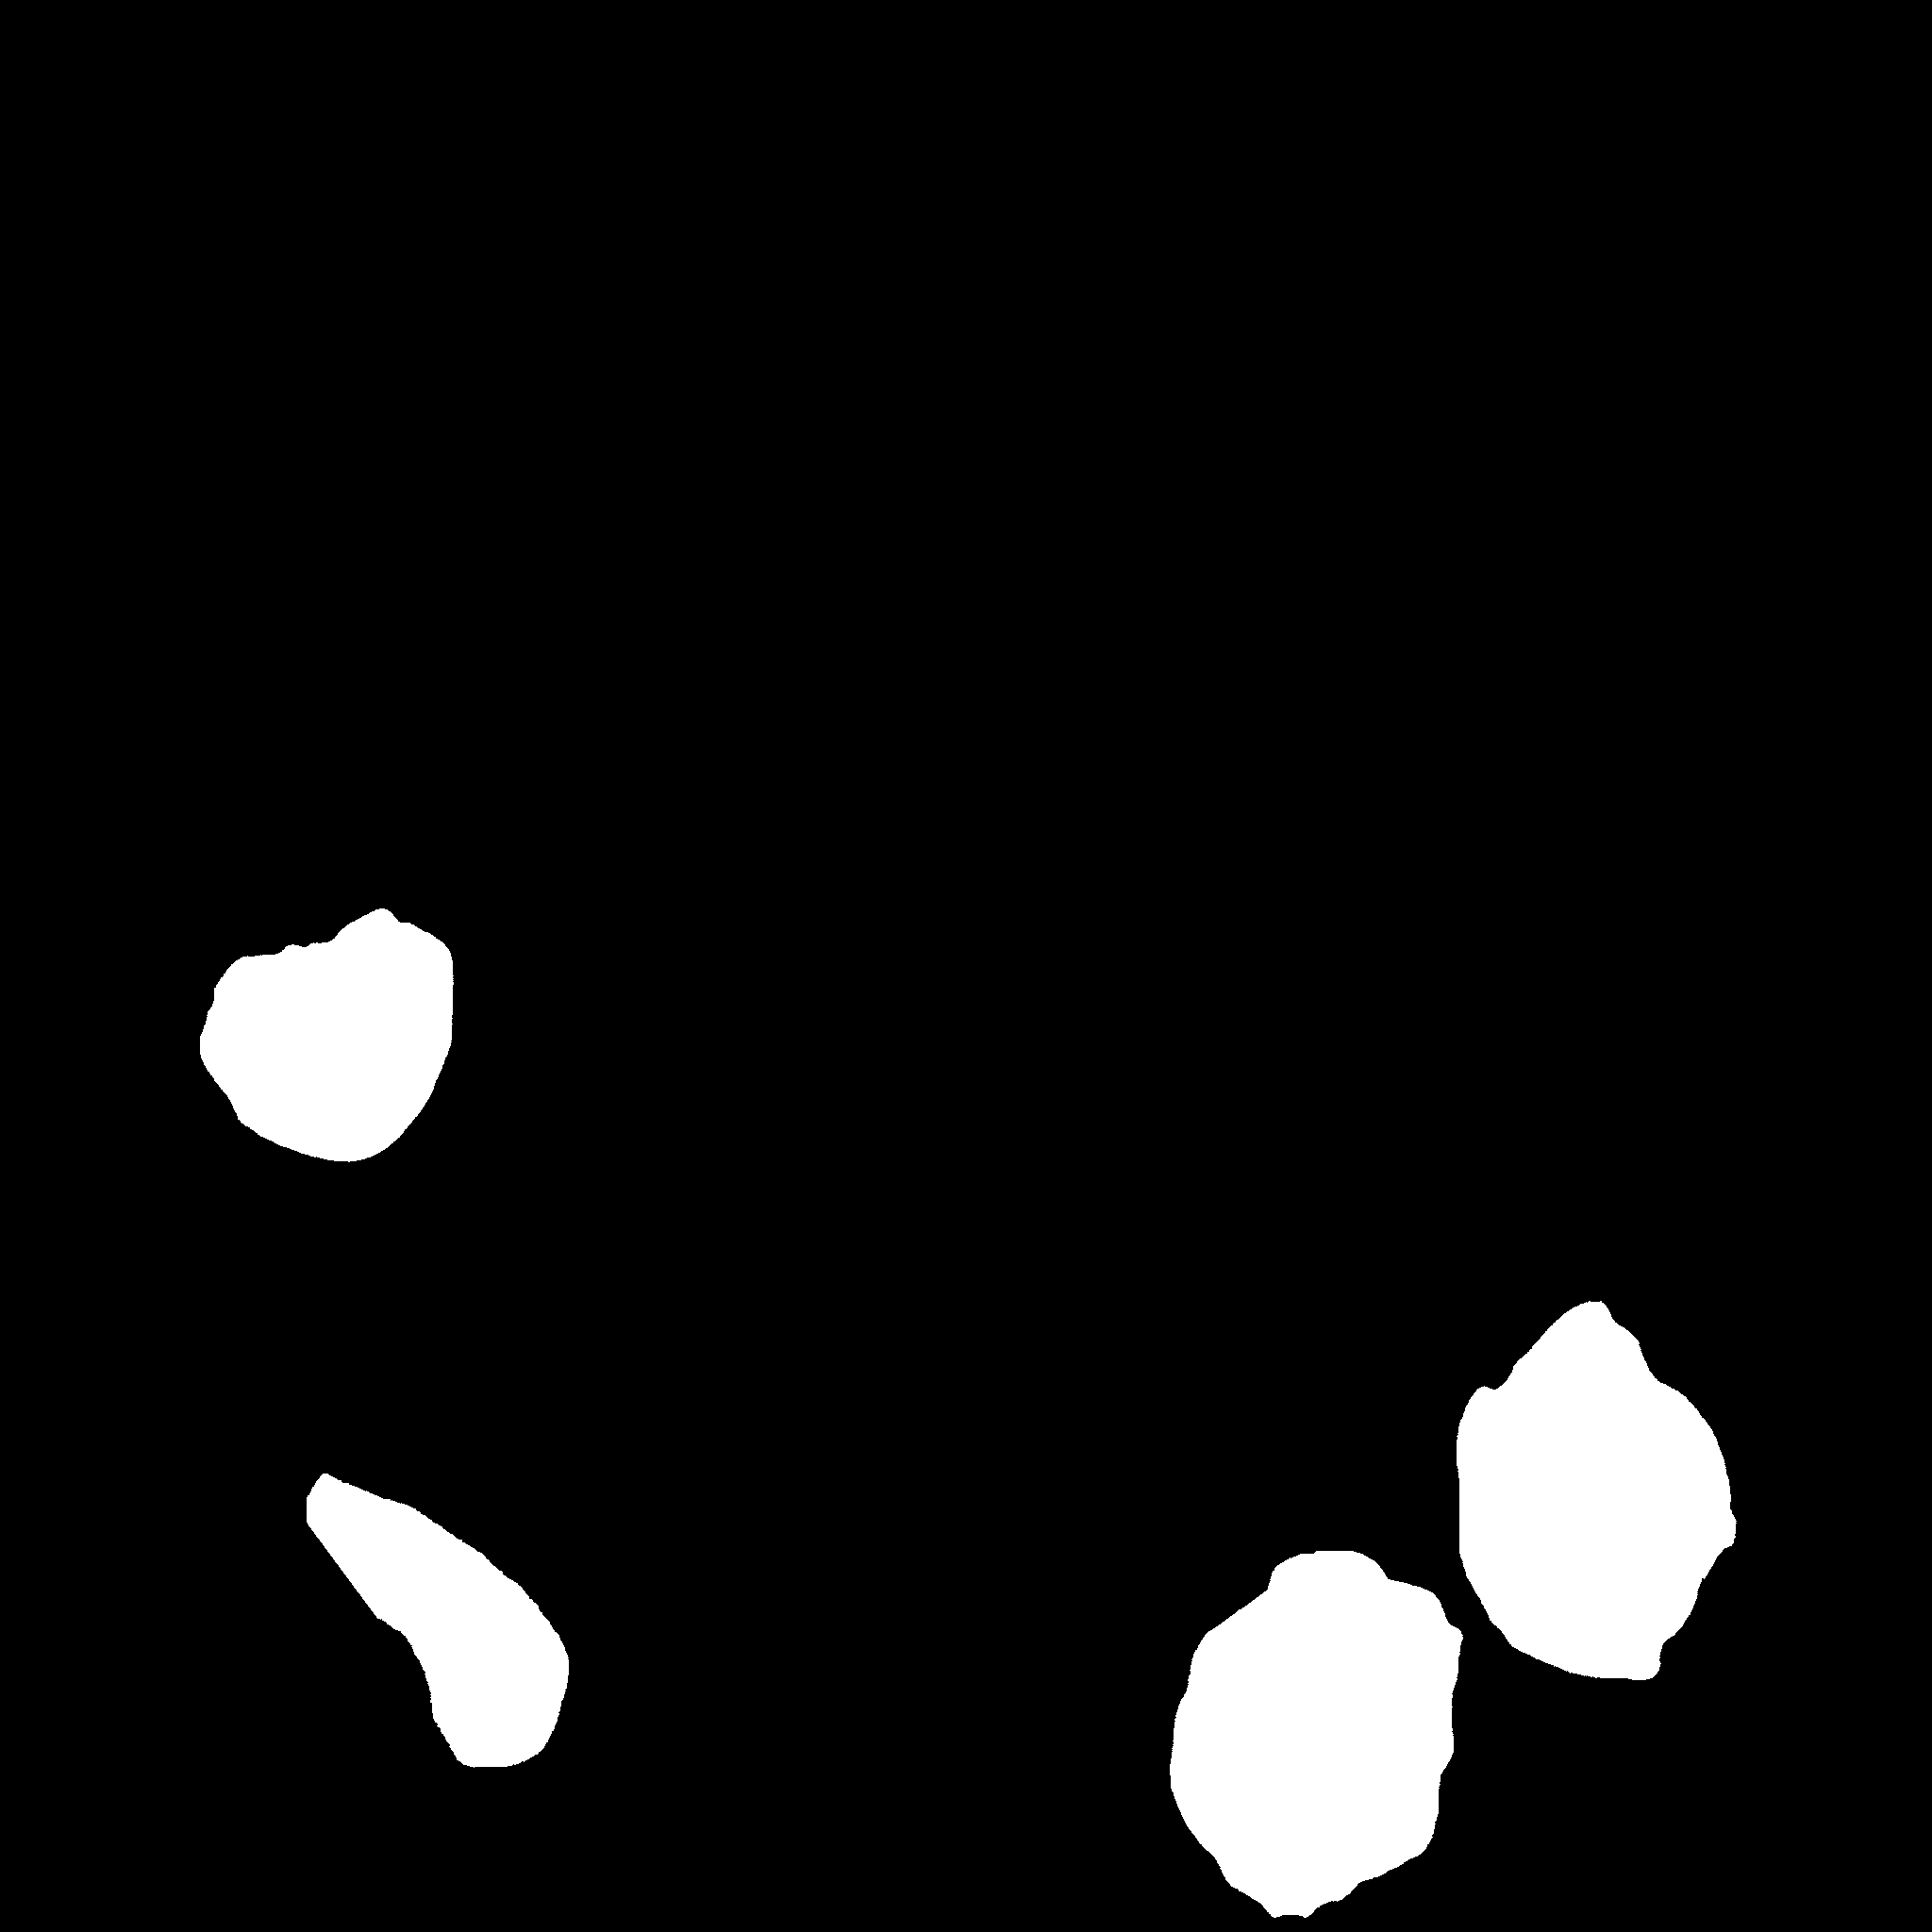
\includegraphics[width = 0.24\textwidth,valign=c]{images/56Nx_12_116_5_5120_0_mask.jpg}
\label{fig_o4}}
\caption{(a) A Whole Slide Image from the training set, and (b) the corresponding manual segmentation. (c) and (d) show a local patch extracted from (a) and its segmentation.}
\label{fig1}
\end{figure}


In the remaining of this paper, we present two segmentation approaches based on encoder-decoder architectures for both patch-level and WSI-level tasks. 
%We experiment with different combinations of encoders and decoders for each task, selecting the optimal model through iterative experimentation. 
We will see how local patch-wise high performance does not necessarily translate into global instance-wise accuracy. 
Indeed, for this specif problem, the model that performed the worse at the local level achieved a widely lower performance at the WSI-level, particularly when considering the task as instance segmentation. 

